\chapter{Methods}

\section{The data}
PLease tell where is the data come from, a little brief of company can be put here.

\section{Method 1}
Definition, steps, algoritm or equation of method 1 and how to apply into your data
\section{Method 2}
Definition, steps, algoritm or equation of method 2 and how to apply into your data


section{Andi Muhammad Aslam/1164064}
\begin{enumerate}

\item Random Forest merupakan algoritma yang digunakan terhadapap klasifikasi data dalam jumlah yang besar. Klasifikasi pada random forest dilakukan dengan penggabungan dicision tree dengan melakukan training terhadap sempel data yang dimiliki. Pembentukan decision tree menggunakan sample data berupa variable secara acak lalu menjalankan klasifikasi pada semua tree yang terbentuk. Random forest berupa Decision Tree agar dapat melakukan proses seleksi. Decision tree yang di buat dibagi secara strategis dari data pada kelas yang sama. Pemecahan digunakan untuk membagi data berdasarkan jenis atribut yang digunakan..  \ref{Andi}

\begin{figure}[ht]
	\centerline{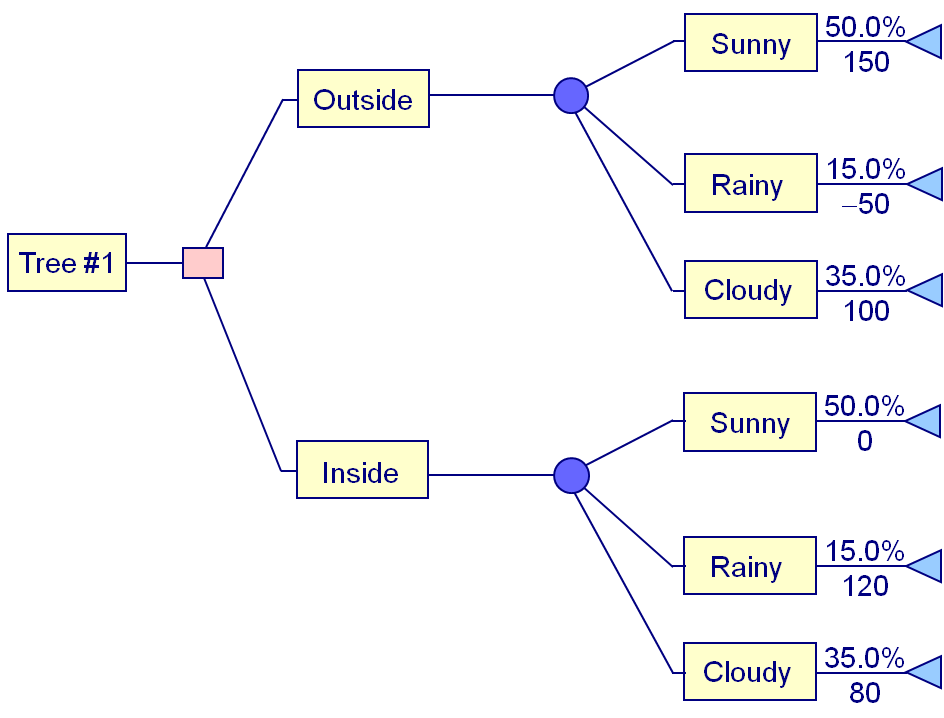
\includegraphics[width=1\textwidth]{figures/andi/decision tree.jpg}}
	\caption{Random Forest.}
	\label{contoh}
	\end{figure}

\item Download dataset terdahulu kemudian buka software spyder untuk melihat isi dataset. Data yang di download berupa extensi file bernama .txt yang terdapat class dari field. Contohnya pada data jenis burung memiliki file index dan angka, dimana index berisi angka yang memiliki makna berupa jenis burung atau bahkan nama burung sedangkan field memiliki isi nilai berupa 0 dan 1 yang dimana sifatnya boolean, Ya dan Tidak. Hal ini dikarenakan komputer hanya dapat membaca bilangan biner maka dari itu field yang di isikan berupa angka. Artinya angka 0 berarti tidak dan angka 1 berarti Ya.

\item Cross validation adalah metode statistik yang digunakan untuk memperkirakan keterampilan model pembelajaran mesin. Ini biasanya digunakan dalam pembelajaran mesin yang diterapkan untuk membandingkan dan memilih model untuk masalah pemodelan prediktif yang diberikan karena mudah dipahami, mudah diimplementasikan, dan menghasilkan estimasi keterampilan yang umumnya memiliki bias lebih rendah daripada metode lainnya.

\item Penjelasan Score
	\begin{itemize}
		\item Pada score 44\% pada random forest berupa hasil akurasi.
		\item Pada score 27\% pada decision tree adalah presentasi hasil dari perhitungan dataset.
		\item Pada  score 29\% dari SVM adalah hasil pendekatan neural network.
		\item Hasil tersebut didapat dari hasil valdasi silang untuk memastikan bahwa membagi  training test dengan cara yang berbeda. Sehingga dapat diketahui hasi output yaitu 44\% untuk hutan, 27\% untuk pohon keputusan, dan 29\% untuk SVM.
	\end{itemize}

\item Untuk membaca confusion matriks dapat menggunakan source code berikut :
	\begin{verbatim}
		import numpy as np
		np.set_printoptions(precision=2)
		plt.figure(figsize=(60,60), dpi=300)
		plot_confusion_matrix(cm, classes=birds, normalize=True)
		plt.show()
	\end{verbatim}

Dimana numpy dapat mengelola data yang berhubungan pada matrix. Pada perintah code tersebut digunakan dalam melakukan read pada dataset burung dengan menggunakan metode confusion matrix. Dalam confusion matrix memiliki 4 istilah yaitu True Positive yang merupakan data posotif yang terditeksi benar, True Negatif yang merupakan data negatif akan tetapi terditeksi benar, False Positif merupakan data negatif namun terditeksi sebagai data positif, False Negatif merupakan data posotif namun terditeksi sebagai data negatif. Adapun contoh hasil read dataset menggunakan confusion matrix dapat dilihat pada figure \ref{Andi}

\item Untuk mengetahui confusion matriks kita dapat melihat contoh klasifikasi dari biner berikut ini :
	\begin{figure}[ht]
	\centerline{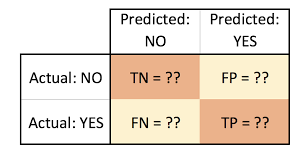
\includegraphics[width=1\textwidth]{figures/andi/CM.PNG}}
	\caption{Tabel Confusion Matriks}
	\label{contoh}
	\end{figure}
\item Voting merupakan proses pemilihan dari tree yang dimana akan dimunculkan hasilnya dan disimpulkan menjadi informasi yang pasti.
	\begin{figure}[ht]
	\centerline{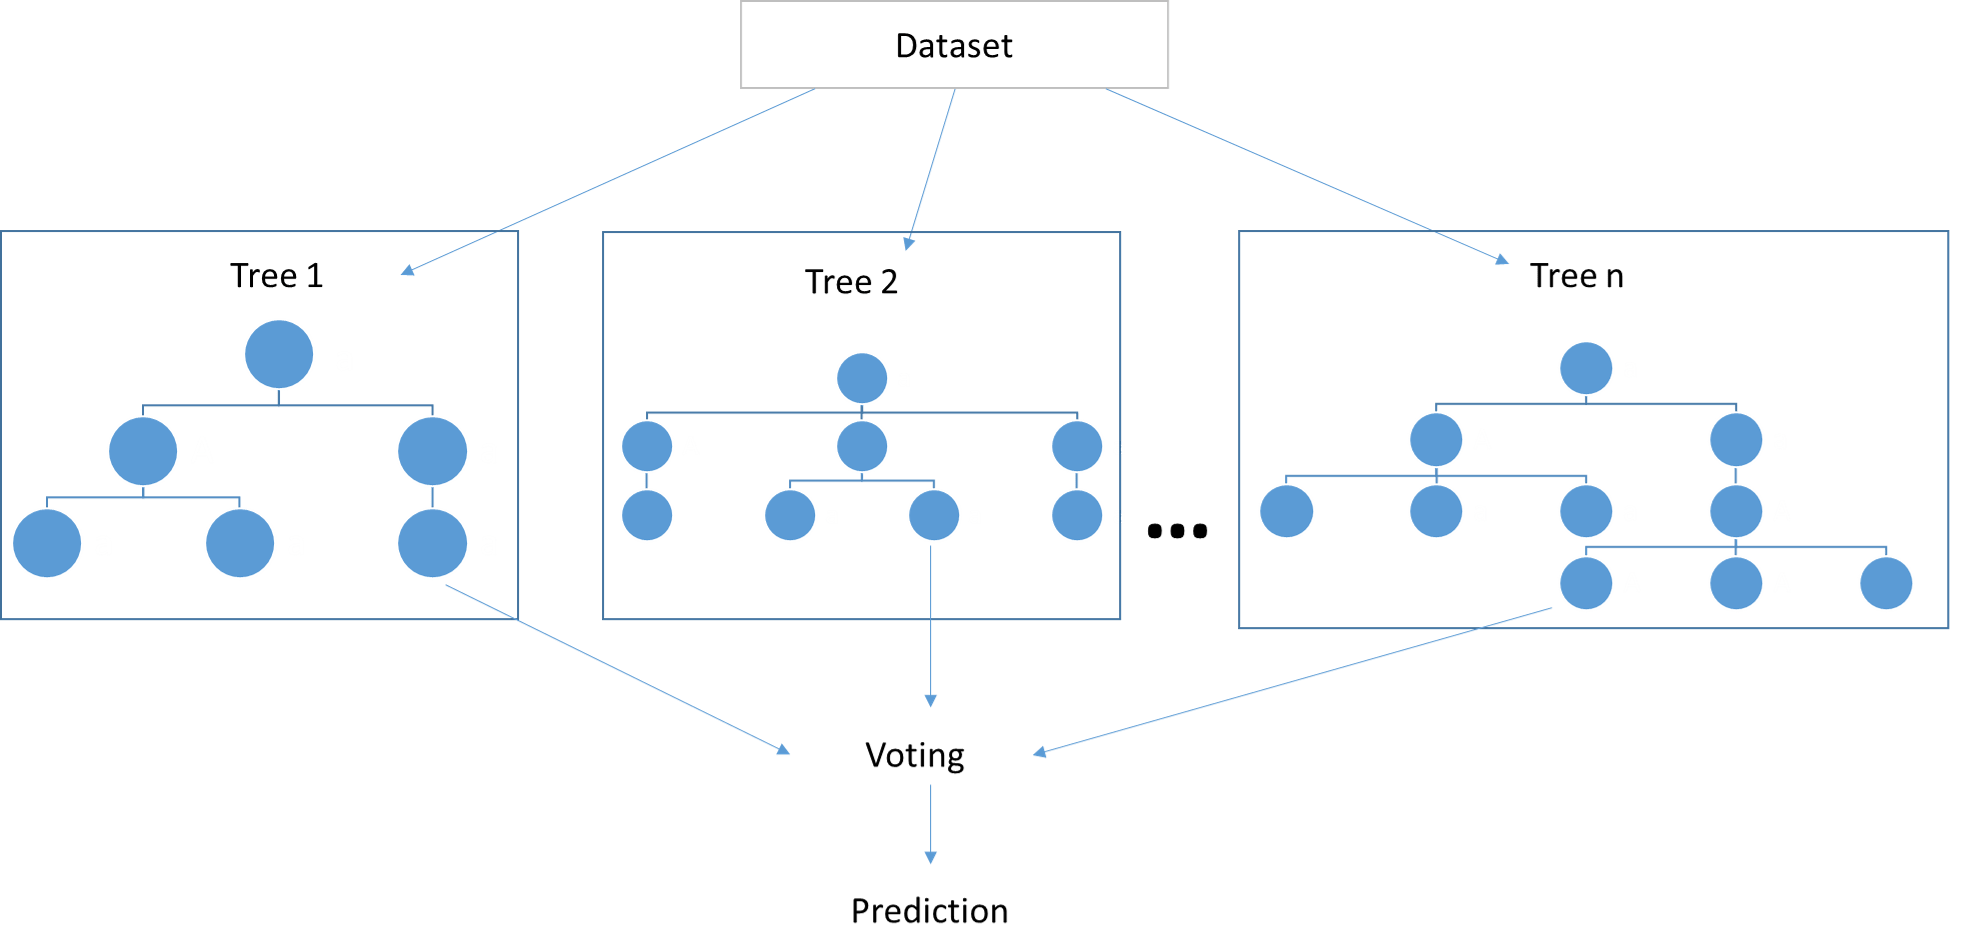
\includegraphics[width=1\textwidth]{figures/andi/Voting.PNG}}
	\caption{Voting}
	\label{Contoh Voting}
	\end{figure}

Pada figure Voting terdapat Decision Tree yang terbagi menjadi 3 Branch yaitu tree 1, tree 2, dan tree 3. Pada tree tersebut akan dilakukan proses voting. Pada  masing-masing tree tersebut memiliki data-data yang berbeda, yang di mana data tersebut akan di pilih dengan cara voting. Hasli voting dari setiap tree tersebut menunjukkan data pada setiap tree, Di sini kita dapat menghitung akurasi dengan menambahkan angka secara diagonal, sehingga ini semua adalah contoh yang diklasifikasikan dengan benar, dan membagi jumlah tersebut dengan jumlah semua angka dalam matriks.

\end{enumerate}